\section{Practical algorithm regimes and worked illustrations}
\label{sec:decision-regimes}
Theorems provide work and storage bounds, but a reader must also
know what changes when the scientific workload changes.
We distinguish a \emph{derived preference under stated assumptions}
from an \emph{observed numerical comparison}. The former cannot
be read off from milliseconds, and the latter cannot establish
an asymptotic ordering.

\subsection{When is SVD preferable, and when is Cholesky?}
\label{sec:which-method}
For a fixed $(n,d)$, a full retained SVD requires
$O(nr^2)$ preprocessing and $O(nr)$ memory ($r=n-d$).
Subsequent projected scalar GCV, AICc, residual BIC and
profiled Gaussian likelihood scores are $O(r)$
per candidate and series after projections. This favors
spectral reuse \emph{conditionally} when $n$ is moderate,
the number $M$ of smoothness values is large, and the
same decomposition serves many observed series or criteria.

A banded Cholesky factorization with an exact
selected-inverse diagnostic instead requires
$O(nd^2)$ arithmetic per penalty and $O(nd)$
working memory at fixed small $d$. It is particularly
attractive for large $n$, small or moderately sized grids,
and memory-constrained problems; the per-candidate
diagnostic is charged even when only the fitted trend
would otherwise be inexpensive. A generic sparse Cholesky
backend can exploit the same structure, but a hybrid
that performs an additional banded factorization should
not be called a pure sparse-Cholesky timing.

For \emph{conditional ordinary CV}, the spectral method
needs the leverage diagonal
$h_i=\sum_{k}v_{ik}^{\,2}/(1+\lambda\delta_k)$ and
the fitted residual vector, costing up to $O(nr)$
per new candidate; the leverage is reusable across
the $R$ series. By contrast, the banded selected-inverse
recursion obtains all $h_i$ with the same $O(nd^2)$
factorization order. Therefore the crossover
for CV need not coincide with the scalar-GCV crossover.
In the fixed-$d$, increasing-$n$ asymptotic regime,
the banded CV path has a structural arithmetic advantage
over the full dense-spectral CV calculation.
Nevertheless, optimized matrix kernels and numerical
tolerances can reverse a \emph{finite-size measured}
ranking. Neither family is universally the fastest.

\begin{figure*}[tbp]\centering
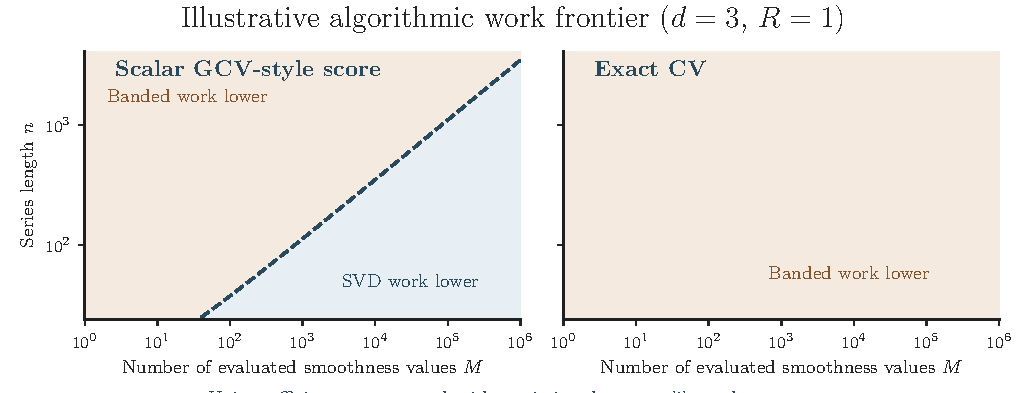
\includegraphics[width=.94\textwidth]{figures/theory_regime_map.pdf}
\caption{Conceptual two-criterion frontier derived from an
explicit \emph{unit-coefficient arithmetic proxy}, not
benchmarked seconds. For $d=3$, $R=1$ and an already mapped
penalty grid, blue denotes lower modeled full-SVD work and
warm shading lower modeled banded-Cholesky work.
The dashed curve is the proxy's equality locus, not a
measured decision boundary. CV includes the dense
leverage and fitted-residual cost; GCV uses scalar
spectral scoring. No numerical conditioning or
hardware-dependent constants are inferred from the shading.}
\label{fig:theory-regime}
\end{figure*}

For a fixed problem size, Proposition~3 permits a
\emph{positive} $M_\star$ only when the SVD has a
larger preparation cost but a strictly smaller
marginal cost of each additional candidate.
Figure~\ref{fig:theory-curves} illustrates both
the possible scalar-criterion crossover and the
absence of one under its chosen CV proxy.
Figure~\ref{fig:theory-regime} similarly provides
an interpretation of the work model, not
a claimed universal machine-level speed classifier.

\begin{figure*}[tbp]\centering
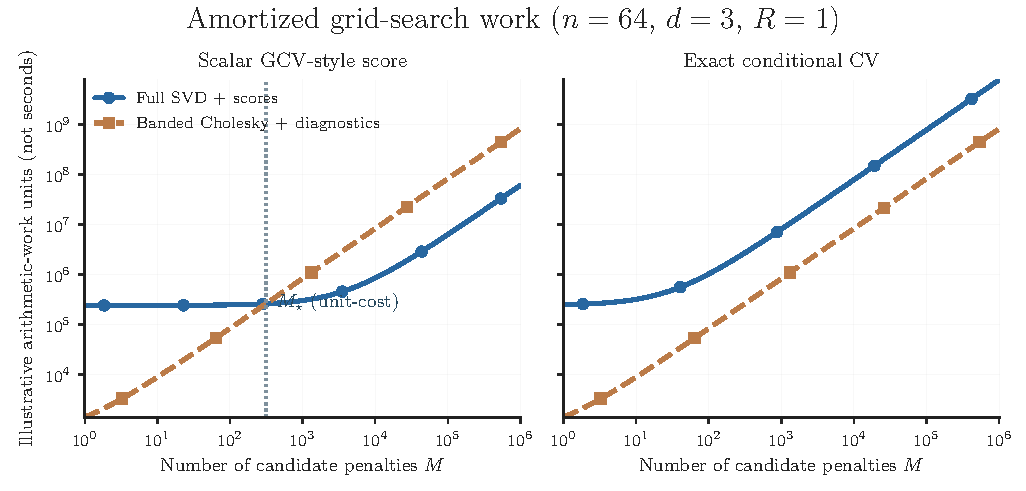
\includegraphics[width=.91\textwidth]{figures/theory_cost_curves.pdf}
\caption{Amortized \emph{operation-work proxies} as $M$ grows,
with $n=64$, $d=3$, $R=1$ and identical premapped
penalties. All leading terms are assigned unit coefficients
for illustration; the marked $M_\star$ in the scalar-score
panel is not an experimentally calibrated runtime
crossover. The CV panel charges full spectral
leverage/residual reconstruction and the
banded selected inverse. Axes are dimensionless
arithmetic counts, not milliseconds.}
\label{fig:theory-curves}
\end{figure*}

\paragraph{Selection policy.}
For a requested full grid, first decide which
\emph{complete} criterion is required. Scalar
spectral scores and classical fixed-$\mu$ CV
do not have the same candidate costs.
Next apply the dense-memory budget before
comparing nominal arithmetic bounds; a
full basis cannot be presumed feasible
for very large $n$. Finally, make the choice
only between numerically admissible pipelines.
An accurate selected-score match in float64
is useful evidence but is not a high-precision
forward-error proof.

\subsection{One reproducible implementation comparison}
\label{sec:matched-example}
A narrowly scoped benchmark illustrates why
the theoretical workload variables matter.
We use the existing archived Windows 11
Experiment010 result for $n=64$, $d=1$,
\[
\widehat\mu=\operatorname{mean}(D_1y),
\qquad
\mathcal S=\{j/10^5:1\le j\le10^5\},
\]
and the source implementation's residual-BIC
score. The end of the grid is the exact
$S=1$ constrained limit; it is not an
attempt to invert an infinite penalty.
Each method executed two recorded repeats for
each of the four one/multiple-candidate,
one/multiple-series workloads and both
\emph{direct-$S$} and already mapped-$\lambda$
coordinates. We report the matched
mapped-$\lambda$ observations below.

All three methods were run sequentially with
one worker and one BLAS thread on the same
university Windows machine, under the same
source revision, seed, candidate set and
numerical criterion. The sparse method is
a \emph{CHOLMOD plus banded selected-inverse}
hybrid, not a pure CHOLMOD factorization.
All 48 raw outcome records have successful
status and matching selected criterion scores
to the recorded tolerance. The comparison
is limited to one $(n,d,\text{criterion})$
configuration and two repeats; it does
not estimate universal crossover thresholds.

\begin{table*}[tbp]
\centering
\caption{Measured median total cold elapsed time
from the \emph{matched single-worker} Windows run.
Single-point times are in milliseconds; the
$10^5$-candidate searches are in seconds.
Each entry is the median of two repeated source
records at fixed $n=64$, $d=1$ and BIC, with
the penalty grid mapped in advance under the
benchmark's stated cold-timing convention.
Do not treat the differing units as a speedup.}
\label{tab:matched-pilot}
\small
\setlength{\tabcolsep}{6pt}
\renewcommand{\arraystretch}{1.16}
\begin{tabular}{@{}lrrrr@{}}
\toprule
& \multicolumn{2}{c}{Single $S$ (ms)}
& \multicolumn{2}{c}{$10^5$ values (s)}\\
\cmidrule(lr){2-3}\cmidrule(l){4-5}
Pipeline & $R=1$ & $R=2$ & $R=1$ & $R=2$\\
\midrule
Full SVD & 2.130 & 2.150 & 8.625 & 9.262\\
Dense inverse & 1.932 & 1.955 & 11.603 & 15.384\\
CHOLMOD hybrid & 2.606 & 2.676 & 32.003 & 37.603\\
\bottomrule
\end{tabular}
\end{table*}

\begin{figure*}[tbp]\centering
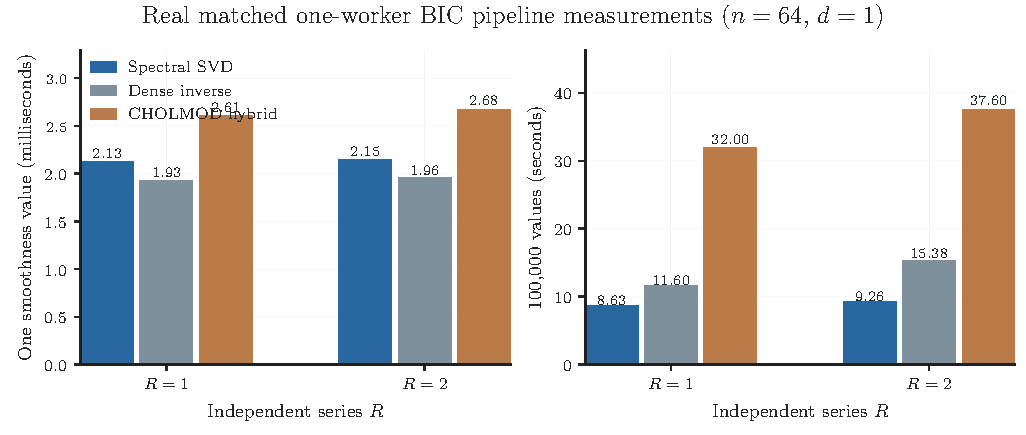
\includegraphics[width=.91\textwidth]{figures/matched_bic_timings.pdf}
\caption{Recorded cold-time medians in Table~\ref{tab:matched-pilot},
recomputed from the 48 original source rows.
Left: one candidate in milliseconds.
Right: $10^5$ candidates in seconds.
All values come from one-worker,
single-BLAS-thread runs. They demonstrate
the benefit of amortized SVD evaluation
for this \emph{particular} BIC configuration;
CV and larger-$n$ conclusions require their
own matched numerical comparisons.}
\label{fig:matched-implementation}
\end{figure*}

The fully auditable CSV is frozen in this
manuscript's \texttt{data/} directory,
with original source SHA and concurrency labels.
It is traceable to the timestamped results branch
described in \texttt{THEORY\_HANDOFF.md}.
The one-worker comparison is an implementation
\emph{example}, not the primary mathematical
contribution of this paper. In particular,
the residual-BIC interpolation boundary may
produce a boundary minimizer rather than a
well-defined unrestricted optimum, so these
runtime measurements must not be interpreted
as evidence that BIC is statistically optimal
for trend forecasting.

\subsection{Real-data illustration: third differences as jerk}
\label{sec:jerk-illustration}
A separate application manuscript in this
repository studies measured longitudinal vehicle
positions from the FHWA NGSIM US-101 dataset
\citep{fhwa2016}.
We reuse only one \emph{predeclared illustrative}
window from that study to demonstrate how a
workload-defined smoothness grid is applied
to a physical signal. The source contains
10-Hz camera-derived positions in meters,
and the training window has $n=80$ observations.
The present illustration uses $d=3$ and
a training-only plug-in difference mean
\[
\widehat\mu
=\frac{1}{n-3}\sum_{t=1}^{n-3}
(D_3y)_t,
\qquad
\frac{D_3\tau}{(\Delta t)^3}
\approx \tau^{(3)}(t).
\]
The latter is a \emph{jerk proxy} for
position sampled at interval $\Delta t=0.1$ s,
not ground-truth jerk from an accelerometer.
The smoothing parameter is the previously
selected GCV grid candidate $S=0.40$,
$\lambda\approx0.08084$, without using
any held-out positions during the selection.
Because $\widehat\mu$ is data-dependent,
its ordinary CV leverage formula would be
conditional rather than an exact refitting
of the plug-in mean.

\begin{figure*}[tbp]\centering
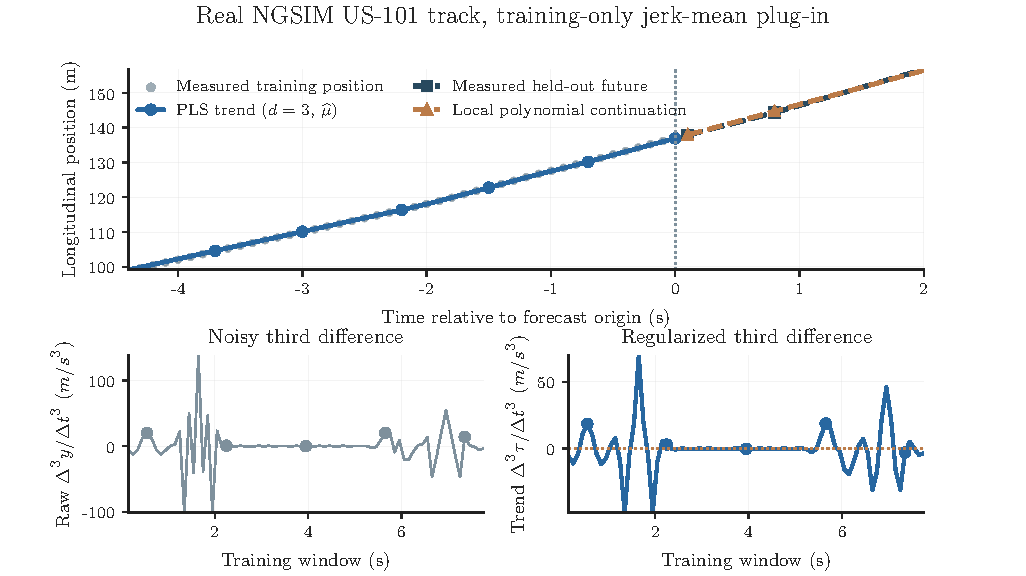
\includegraphics[width=.94\textwidth]{figures/ngsim_jerk_application.pdf}
\caption{One real US-101 trajectory, reused from
the separate NGSIM jerk case study. Upper
panel: the last 45 measured training positions,
$d=3$ PLS fit with training-derived
$\widehat\mu$, measured future positions
held out during fitting, and a
\emph{separately appended} local-polynomial
continuation over two seconds.
Lower panels: noisy third differences of
observations and of the regularized trend,
on their individual vertical scales.
These curves do not establish a true
jerk value or a PLS-intrinsic forecast.}
\label{fig:jerk-application}
\end{figure*}

PLS itself estimates the historical trend
and does \emph{not} produce the forecast
in Figure~\ref{fig:jerk-application}. The
companion study obtains future positions
by fitting a local polynomial of degree
$d-1$ to the last 25 fitted positions
after removing the particular solution
$\widehat\mu\binom{t}{d}$, then restoring
that particular solution at the future
indices. The holdout comprises 20
chronological frames, and no model is
fitted to those future observations.
The full evaluation, physical baselines
and the distinct forecasting objectives
belong to
\texttt{paper/ngsim-jerk-case-study/};
the present paper uses only the
illustration to connect its abstract
cost variables to a concrete
time-series workload. Numerical
differentiation of noisy observations
is itself an ill-posed estimation
problem, as discussed by
\citet{vanbreugel2020}.

